% Copyright 2026 Sreeram Anil
% SPDX-License-Identifier: CC-BY-4.0
\chapter{Unscented particle filter (UPF)}
\label{ch:upf}

\section*{At a glance}
\begin{tabular}{@{}l>{\raggedright\arraybackslash}p{0.76\textwidth}@{}}
Family & Sequential Monte Carlo (particle / ensemble / Gaussian sum) \\
Header & \texttt{include/estkit/particle/upf.hpp} \\
Registered name & \texttt{UPF} ($N=30$ particles, one UKF measurement update each) \\
State dimension & $n_x = 4$ (cell model) — generic in $n_x, n_u, n_y$ \\
Cost per step & \SI{18.6}{\micro\second}/step ($39\times$ EKF); $N(2n_x{+}1)$ evaluations of $h$ \\
Memory & \SI{25.3}{\kilo\byte} (particles, per-particle covariances, one UKF workspace) \\
Primary references & \cite{vandermerwe2000upf,doucet2000smc,wan2000ukf,julier2004unscented} \\
\end{tabular}

\section{Motivation and aerospace/BMS relevance}
The bootstrap filter proposes blindly.  Chapter~\ref{ch:pfauxiliary} repairs that by choosing
\emph{which} particle to propagate using the new measurement; this chapter repairs it by choosing
\emph{where} to propagate each particle, again using the new measurement.  The two ideas are
complementary and the second is the more powerful of the two, because it moves the samples rather
than merely re-weighting them.

Doucet, Godsill and Andrieu \cite[\S{}II-B]{doucet2000smc} show that the importance density which
minimises the conditional variance of the weights is the \emph{optimal importance density}
\begin{equation}
  q_{\mathrm{opt}}(\vx_k\mid\vx_{k-1}^i,\vy_k) \;=\; p(\vx_k\mid\vx_{k-1}^i,\vy_k)
  \;\propto\; p(\vy_k\mid\vx_k)\,p(\vx_k\mid\vx_{k-1}^i),
  \label{eq:upf-qopt}
\end{equation}
which for a nonlinear $h$ has no closed form.  van der Merwe, Doucet, de Freitas and Wan
\cite{vandermerwe2000upf} approximate it by running an \emph{unscented Kalman} measurement update
per particle and proposing from its Gaussian posterior.  The sigma-point machinery is used exactly
as in the UKF chapter of the Kalman family, but its output is not the estimate --- it is a proposal, and the
importance weights correct whatever error the unscented approximation makes.  The filter is thus
"a UKF that knows it is approximate": the Gaussian assumption is used where it is cheap and helpful,
and audited by the Monte-Carlo layer.

In aerospace this is the standard recipe when measurements are precise and expensive to waste:
star-tracker-aided attitude, radar track initiation, GNSS re-acquisition.  For a battery, the
voltage sensor resolves SOC to \num{0.003} while the one-step SOC uncertainty is $10^{-5}$ --- a
ratio of \num{300} --- so blind proposal is maximally wasteful and a measurement-aware one should
pay off.  The chapter quantifies when it does, and documents a failure mode of the original
formulation that is specific to models with very small process noise.

\section{Problem statement and assumptions}
Model \eqref{eq:pfb-dyn}--\eqref{eq:pfb-meas} as before, plus
\begin{quote}
(A5) $h$ is smooth enough for the unscented transform to give a usable Gaussian approximation of
$p(\vy_k\mid\vx_k)$ over the support of the one-step predictive, and the resulting proposal has
heavier tails than the target in every direction (so that the importance weights are bounded).
\end{quote}
(A5) is not a mild assumption.  A proposal narrower than the target produces unbounded weights and
is the classical way to destroy an importance sampler; the practical safeguard is that the UKF
posterior covariance is always smaller than its prior, so the prior must itself be a valid
envelope of the transition density.  That requirement drives the central design decision of this
implementation, discussed next.

\section{Derivation}

\subsection{The proposal}
Particle $i$ enters the step as a \emph{point} $\vx_{k-1}^i$, not as a distribution.  Its exact
one-step predictive is therefore the transition density itself,
\begin{equation}
  p(\vx_k\mid\vx_{k-1}^i) \;=\; \N{f(\vx_{k-1}^i,\vu_{k-1})}{\mQ_{\mathrm{eff}}}
  \;=\; \N{\bm{\mu}^i}{\mQ_{\mathrm{eff}}},
  \label{eq:upf-prior}
\end{equation}
with no approximation whatsoever.  Applying an unscented \emph{measurement} update to
\eqref{eq:upf-prior} yields a Gaussian approximation of the optimal density \eqref{eq:upf-qopt}:
with sigma points $\{\mathcal{X}_s\}$ drawn from $(\bm\mu^i, \mQ_{\mathrm{eff}})$ and weights
$W_s^m, W_s^c$ as in the UKF chapter of the Kalman family,
\begin{align}
  \yhat^i &= \sum_s W^m_s\, h(\mathcal{X}_s,\vu_k), &
  \mP^i_{yy} &= \mR + \sum_s W^c_s (h(\mathcal{X}_s,\vu_k)-\yhat^i)(\cdot)^\T, \label{eq:upf-ut1}\\
  \mP^i_{xy} &= \sum_s W^c_s (\mathcal{X}_s - \bm\mu^i)(h(\mathcal{X}_s,\vu_k)-\yhat^i)^\T, &
  \mK^i &= \mP^i_{xy}(\mP^i_{yy})\inv, \label{eq:upf-ut2}\\
  \vx_a^i &= \bm\mu^i + \mK^i(\vy_k - \yhat^i), &
  \mP_a^i &= \mQ_{\mathrm{eff}} - \mK^i\mP^i_{yy}(\mK^i)^\T, \label{eq:upf-ut3}
\end{align}
and the proposal is
\begin{equation}
  q(\vx_k\mid\vx_{k-1}^i,\vy_k) = \N{\vx_a^i}{\mP_a^i}, \qquad
  \vx_k^i = \vx_a^i + \mL_a^i\bm\xi^i, \quad \mL_a^i(\mL_a^i)^\T = \mP_a^i, \quad \bm\xi^i\sim\N{\bm 0}{\mI}.
  \label{eq:upf-draw}
\end{equation}

\subsection{The weight}
Nothing cancels in the general SIS recursion \eqref{eq:pfb-sis}, so all three densities must be
evaluated:
\begin{equation}
  \boxed{\;
  \log \tilde w_k^i = \log \tilde w_{k-1}^i
    + \underbrace{\log \N{\vy_k - h(\vx_k^i,\vu_k)}{\mR}}_{\text{likelihood}}
    + \underbrace{\log \N{\vx_k^i - \bm\mu^i}{\mQ_{\mathrm{eff}}}}_{\text{transition}}
    - \underbrace{\log \N{\vx_k^i - \vx_a^i}{\mP_a^i}}_{\text{proposal}} \;}
  \label{eq:upf-weight}
\end{equation}
The proposal term is free: because $\vx_k^i$ was generated as $\vx_a^i + \mL_a^i\bm\xi^i$, the
Mahalanobis distance is exactly $\norm{\bm\xi^i}^2$ and the log-determinant is
$\sum_k \log (\mL_a^i)_{kk}$, both already available.  The transition term needs one triangular
solve against the shared factor of $\mQ_{\mathrm{eff}}$.

If the unscented approximation were exact, \eqref{eq:upf-weight} would collapse to
$\log\tilde w^i_k = \log\tilde w^i_{k-1} + \log p(\vy_k\mid\vx^i_{k-1})$, i.e.\ the incremental
weight would be the \emph{predictive} likelihood of the parent, independent of the draw
$\bm\xi^i$ --- zero conditional weight variance, the definition of the optimal proposal.  What the
filter actually pays is the mismatch between the unscented Gaussian and the true conditional.

\subsection{Why the per-particle covariance of the original formulation fails here}
van der Merwe et al.\ carry a covariance $\mP^i$ with every particle and propagate it with a
\emph{full} UKF (time update and measurement update), so that the proposal prior is
$\N{\text{UKF-predicted }\vx^i}{\mP^i_{k|k-1}}$ rather than \eqref{eq:upf-prior}.  Each particle
then represents a local Gaussian rather than a point.  That is a legitimate and often superior
variant --- it is available as \code{Options::carry\_covariance} --- but on this model it breaks
the weight recursion.  The reason is quantitative.  All $N$ per-particle UKFs see the same
measurements, so their covariances converge to the same Kalman steady state, whose SOC standard
deviation is $\sqrt{(\mP)_{\soc\soc}} \approx 1.1\times10^{-3}$.  The transition density in
\eqref{eq:upf-weight}, however, has SOC standard deviation
$\sqrt{q_{\soc}} = 10^{-5}$.  A draw from the proposal therefore lands routinely $100$ standard
deviations into the tail of the transition density, the term
$\log\N{\vx^i_k-\bm\mu^i}{\mQ}$ is of order $-5000$ and varies by hundreds of nats between
particles, and every step the whole weight mass collapses onto one particle.  Measured on the
nominal eVTOL mission (development run, seed 1): $\mathrm{RMSE}_{\mathrm{ss}} =
\SI{3.5}{\percent}$ with a voltage-residual RMSE of \SI{3.6}{\milli\volt}, i.e.\ more than an order
of magnitude worse than the bootstrap filter.

The default configuration avoids this by treating a particle as what it is --- a sample --- so that
the proposal prior is the exact transition density, and by folding the roughening jitter into that
same density:
\begin{equation}
  \mQ_{\mathrm{eff}} = \mQ(\xhat,\vu_{k-1}) + \diag(\sigma_1^2,\dots,\sigma_{n_x}^2),
  \qquad \sigma_k \text{ from } \eqref{eq:pfb-roughen-clip}.
  \label{eq:upf-qeff}
\end{equation}
Both the proposal \eqref{eq:upf-ut3} and the transition term in \eqref{eq:upf-weight} then use the
\emph{same} $\mQ_{\mathrm{eff}}$, the recursion stays exact for the jittered model, and the weights
are well behaved.  This is also what makes the UPF worth its cost here: with
$\varphi_{\max} = 0.02$ the effective SOC process standard deviation is
$2\times10^{-3}$, comparable to the \num{0.003} that the likelihood resolves, so the unscented
update actually \emph{moves} the proposal --- the SOC gain in \eqref{eq:upf-ut3} is about
\num{0.44}, against $1.6\times10^{-5}$ if the raw $\mQ$ were used.  With the raw $\mQ$ the optimal
proposal coincides with the prior and the UPF degenerates, correctly but uselessly, into an
$N=30$ bootstrap filter.  Carrying the per-particle covariance is measured (same development run) at
$\mathrm{RMSE}_{\mathrm{ss}} = \SI{1.2}{\percent}$ against \SI{0.7}{\percent} for the default.

\section{Algorithm}
\begin{algorithm}[H]
\caption{UPF --- one sampling period}
\begin{algorithmic}[1]
\Require particles $\{\vx_{k-1}^i\}$, log-weights $\{\ell^i\}$, $\vu_{k-1},\vu_k,\vy_k$
\State \textbf{Time update (\code{predict}).}
\State $\bm\sigma \gets$ roughening scale \eqref{eq:pfb-roughen-clip}; \; $\mQ_{\mathrm{eff}} \gets \mQ(\xhat,\vu_{k-1}) + \diag(\bm\sigma^2)$; \; $\mL_Q \gets \operatorname{chol}(\mQ_{\mathrm{eff}})$
\For{$i=1$ \textbf{to} $N$} \State $\bm\mu^i \gets f(\vx_{k-1}^i,\vu_{k-1})$ \EndFor
\State \textbf{Prior predictive.} $\yhat_k \gets \sum_i w^i h(\bm\mu^i,\vu_k)$
\State \textbf{Measurement update (\code{update}).}
\For{$i=1$ \textbf{to} $N$}
  \State unscented update of $(\bm\mu^i,\mQ_{\mathrm{eff}})$ with $\vy_k$ $\to$ $(\vx_a^i,\mP_a^i)$ \Comment{eqs. \eqref{eq:upf-ut1}--\eqref{eq:upf-ut3}}
  \State $\mL_a \gets \operatorname{chol}(\mP_a^i)$; \; $\bm\xi^i \sim \N{\bm 0}{\mI}$; \; $\vx_k^i \gets \operatorname{constrain}(\vx_a^i + \mL_a\bm\xi^i)$
  \State $\log q \gets -\tfrac12\norm{\bm\xi^i}^2 - \sum_m \log(\mL_a)_{mm} - \tfrac{n_x}{2}\log 2\pi$
  \State $\ell^i \gets \ell^i + \log\N{\vy_k - h(\vx_k^i,\vu_k)}{\mR} + \log\N{\vx_k^i-\bm\mu^i}{\mQ_{\mathrm{eff}}} - \log q$
\EndFor
\State normalise $\{\ell^i\}\to\{w^i\}$; \; $N_{\mathrm{eff}}\gets 1/\sum_i (w^i)^2$
\If{$N_{\mathrm{eff}} < \beta N$} \State systematic resampling; \; $w^i \gets 1/N$ \EndIf
\State $\xhat_k \gets \sum_i w^i\vx_k^i$; \; $\mP_k \gets \sum_i w^i(\vx_k^i-\xhat_k)(\vx_k^i-\xhat_k)^\T$
\Ensure $\xhat_k$, $\mP_k$
\end{algorithmic}
\end{algorithm}

\noindent At $k=0$ there is no time update; the filter then performs a plain importance-sampling
weighting of the prior cloud, which is the correct degenerate case (the prior \emph{is} the
predictive).

\section{Application to the battery model}
Each of the $N=30$ particles triggers one sigma-point set of $2n_x+1 = 9$ points and therefore
$9$ evaluations of the terminal-voltage map $h$, plus three $4\times4$ Cholesky factorisations
(sigma points, proposal draw, transition density --- the last one shared).  Against the cell model
that is \num{270} evaluations of $h$ per step, each containing one exponential for $R_0(T)$, which
is cheaper than the $500$ evaluations of $f$ (seven exponentials each) that the bootstrap filter
performs.  The measured \SI{18.6}{\micro\second}/step is consequently close to
\estname{PF-Fast}'s \SI{16.0}{\micro\second} and \SI{24}{\percent} of \estname{PF-Bootstrap}'s
\SI{76.4}{\micro\second} --- the UPF is not expensive \emph{per step} here, it is expensive
\emph{per particle}, which is why $N$ is set to 30.

The design trade is visible in the numbers: 30 measurement-aware particles buy rather less accuracy
than 100 blind ones (\SI{0.38}{\percent} against \SI{0.18}{\percent} on \code{nominal}), because
the proposal's advantage is partially spent on the weight correction \eqref{eq:upf-weight} and
because a 30-particle cloud has very thin tails --- the transient peak error in \code{init\_error}
is \SI{11.5}{\percent}, the largest of the family.

\section{Implementation notes}
\emph{One UKF instance, not $N$.}  A \code{Ukf<Model>} object contains a copy of the model (the OCV
table alone is \SI{3.9}{\kilo\byte}); instantiating one per particle would cost \SI{140}{\kilo\byte}
for $N=30$.  Since the UKF is a pure function of $(\vx,\mP)$ between calls, the header keeps a
single instance as a workspace and re-initialises it for every particle.  Memory is then
\SI{25.3}{\kilo\byte}, dominated by the $N$ stored covariances (which only the
\code{carry\_covariance} variant actually needs).

\emph{Scaled unscented transform.}  The default $\alpha = 0.1$, $\beta = 2$, $\kappa = 0$ of
\code{Ukf} is inherited, and exposed through \code{Options} so that the proposal can be widened
independently of the UKF used elsewhere.  With $\alpha$ this small the zeroth weight is strongly
negative ($W_0^c \approx -96$) and $\mP_a^i$ can lose positive definiteness; \code{cholesky\_safe}
adds diagonal jitter in that case, which errs in the safe direction (a slightly too wide proposal).

\emph{Reported covariance.}  $\mP_k$ is the weighted sample covariance of the cloud \emph{after}
resampling.  Unlike the other particle filters in this family the UPF applies no post-resampling
jitter (its roughening lives in $\mQ_{\mathrm{eff}}$ and therefore acts at the next proposal), so on
a step where the 30 particles collapse onto a single parent the reported \code{soc\_std} is exactly
zero for that one sample before the next proposal re-disperses them.  The $\pm2\sigma$ band in the
figures below therefore pinches shut occasionally; this is an artefact of the representation, not a
claim of perfect knowledge.

\emph{Guard on the proposal.}  When \code{apply\_constraints} is on, the drawn particle is projected
onto the feasible set \emph{after} the proposal density has been evaluated, so $\log q$ refers to
the unprojected draw.  Strictly this makes the proposal a projected Gaussian and the weight
slightly inexact; the alternative (rejecting and redrawing) would break the constant-time
guarantee.  The bias is confined to particles that would have left $\soc\in[-0.05,1.05]$, which in
practice happens only in the first steps of the \code{init\_error} scenario.

\section{Benchmark results}
% Copyright 2026 Sreeram Anil
% SPDX-License-Identifier: CC-BY-4.0
\begin{table}[H]\centering\footnotesize\setlength{\tabcolsep}{4pt}
\caption{UPF: cell-level benchmark on the eVTOL mission (mean over seeds; RMSE and max error in \% SOC; $t_\mathrm{conv}$: first time the error stays below 2\,\% for 60\,s, -- = never; EKF reference: steady-state RMSE of the plain EKF on the same data).}\label{tab:cell_UPF}
\begin{tabular}{llrrrrrcrr}\toprule
plant & scenario & RMSE & RMSE$_\mathrm{ss}$ & max & $t_\mathrm{conv}$ [s] & RMSE$_v$ [mV] & div. & EKF ref. & ns/step \\ \midrule
ECM & nominal & 0.60 & 0.38 & 3.76 & 0 & 1.27 & no & 0.05 & 18614 \\
ECM & init\_error & 0.71 & 0.41 & 11.49 & 69 & 2.47 & no & 0.05 & 18528 \\
ECM & current\_bias & 1.10 & 0.99 & 4.51 & 0 & 1.28 & no & 0.61 & 18594 \\
ECM & noise\_step & 0.86 & 0.86 & 3.87 & 0 & 5.47 & no & 0.12 & 18603 \\
ECM & outliers & 0.76 & 0.61 & 4.29 & 260 & 3.67 & no & 0.21 & 18523 \\
ECM & cold & 1.12 & 0.74 & 5.60 & 0 & 2.21 & no & 0.16 & 18713 \\
ECM & hot & 0.35 & 0.29 & 2.76 & 0 & 1.13 & no & 0.03 & 18605 \\
ECM & aged\_cell & 3.60 & 2.74 & 15.99 & 479 & 2.72 & no & 1.52 & 18639 \\
ECM & param\_mismatch & 2.51 & 1.81 & 13.79 & 1 & 2.18 & no & 1.36 & 18540 \\
ECM & sensor\_dropout & 0.68 & 0.49 & 6.62 & 0 & 2.00 & no & 0.46 & 18596 \\
ECM & preisach & 1.65 & 1.16 & 6.14 & 219 & 1.29 & no & 0.20 & 18653 \\
ECM & combined & 3.55 & 2.64 & 18.63 & 544 & 3.61 & no & 12.44 & 18473 \\
\midrule
SPM & nominal & 1.70 & 1.07 & 5.83 & 272 & 1.31 & no & 3.73 & 18342 \\
SPM & init\_error & 1.61 & 0.84 & 11.49 & 425 & 2.36 & no & 3.81 & 18375 \\
SPM & current\_bias & 1.84 & 1.71 & 6.26 & 252 & 1.36 & no & 5.69 & 18447 \\
SPM & noise\_step & 1.83 & 1.44 & 5.83 & 272 & 5.58 & no & 3.30 & 18173 \\
SPM & outliers & 1.42 & 1.32 & 6.56 & 283 & 3.69 & no & 1.99 & 18440 \\
SPM & cold & 4.42 & 5.04 & 15.89 & 542 & 3.68 & no & 7.35 & 18563 \\
SPM & hot & 1.79 & 1.42 & 6.39 & 273 & 1.14 & no & 2.16 & 18401 \\
SPM & param\_mismatch & 2.93 & 1.89 & 11.36 & 713 & 1.68 & no & 3.13 & 18298 \\
SPM & sensor\_dropout & 1.81 & 1.34 & 8.48 & 280 & 2.25 & no & 5.31 & 18439 \\
\bottomrule\end{tabular}\end{table}

\begin{figure}[H]\centering
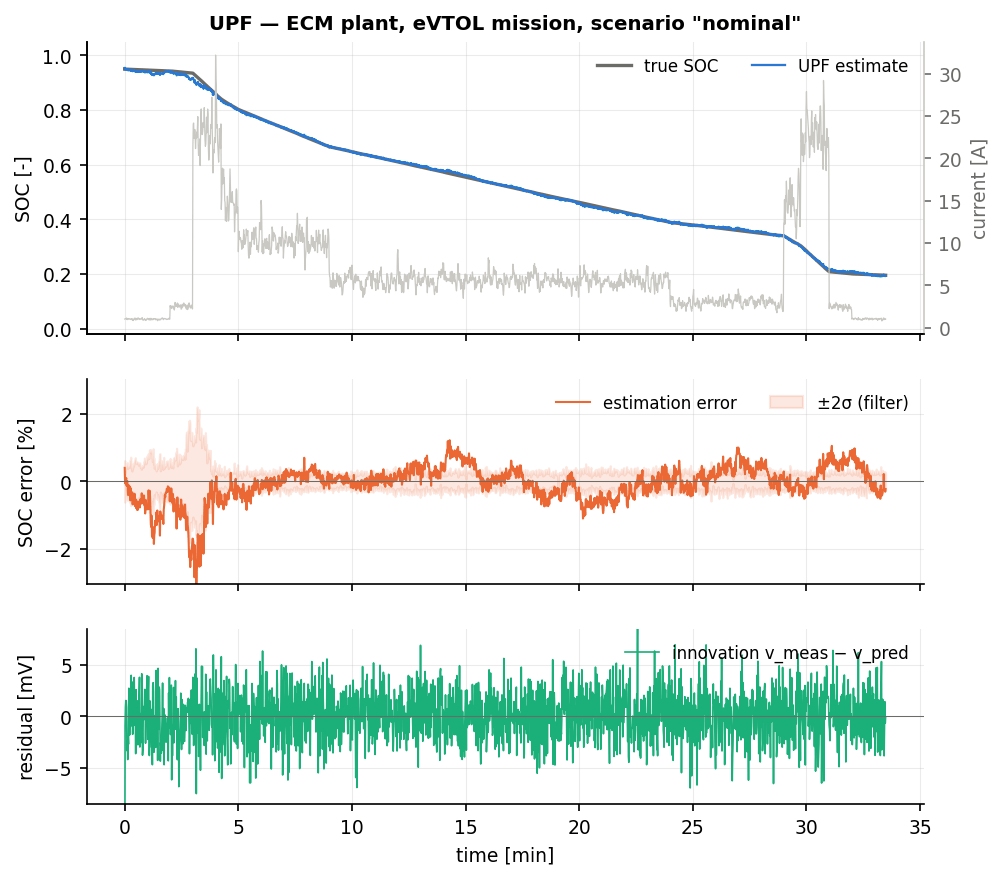
\includegraphics[width=\textwidth]{figures/cell_UPF_nominal.png}
\caption{UPF on the nominal eVTOL mission: true and estimated SOC (top), estimation error with the
$\pm2\sigma$ band (middle), voltage residual (bottom).  The residual noise reflects the small cloud
($N=30$).}
\end{figure}
\begin{figure}[H]\centering
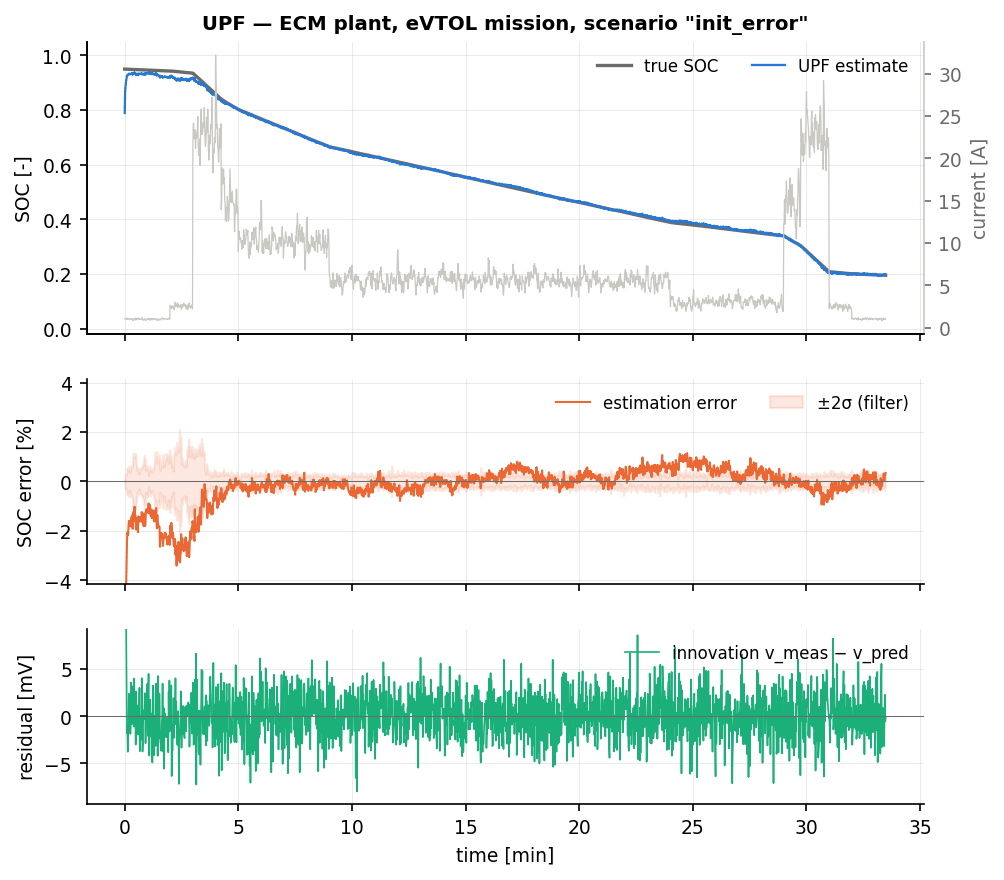
\includegraphics[width=\textwidth]{figures/cell_UPF_init_error.png}
\caption{UPF with a \SI{35}{\percent} initial SOC error.  The measurement-aware proposal pulls the
30 particles towards the truth within a few steps, but the small cloud produces the largest
transient peak of the family (\SI{11.5}{\percent}).}
\end{figure}
\begin{figure}[H]\centering
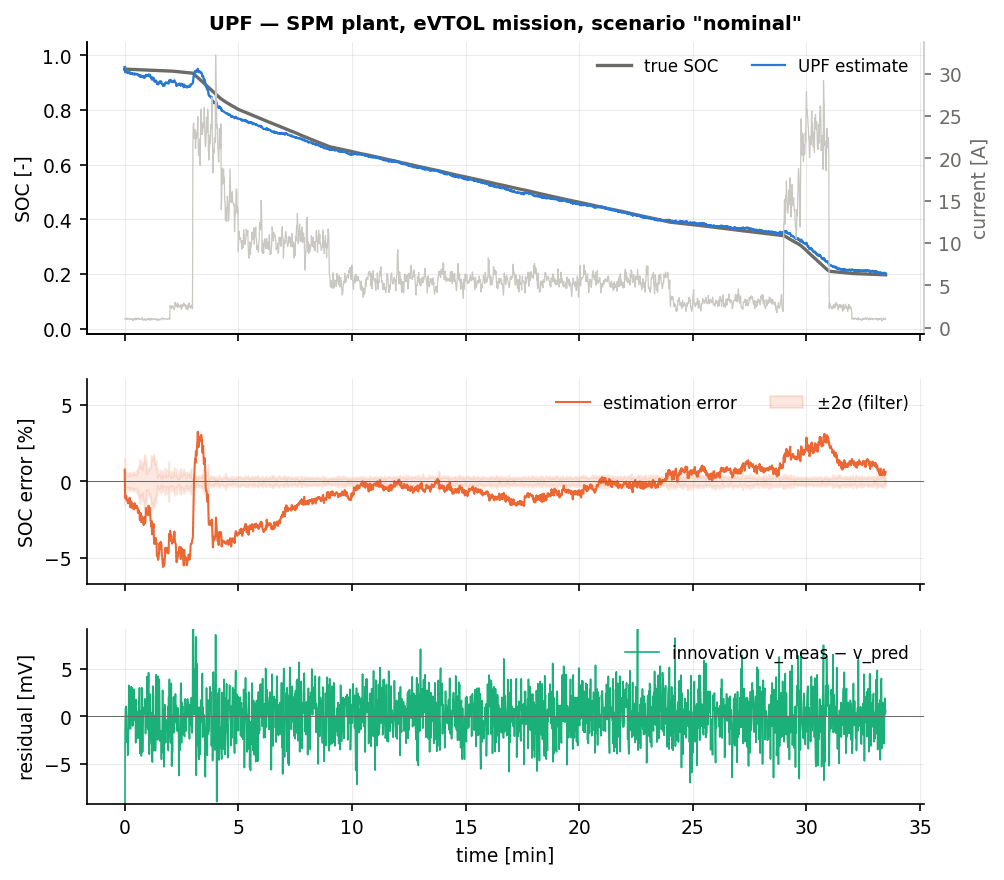
\includegraphics[width=\textwidth]{figures/cellspm_UPF_nominal.png}
\caption{UPF on the electrochemical (SPM) plant, nominal mission: \SI{1.07}{\percent} against
\SI{3.73}{\percent} for the EKF, with thirty particles.}
\end{figure}

\paragraph{ECM plant.}  On \code{nominal} the UPF reaches $\mathrm{RMSE} = \SI{0.60}{\percent}$,
$\mathrm{RMSE}_{\mathrm{ss}} = \SI{0.38}{\percent}$, maximum error \SI{3.76}{\percent}, immediate
convergence and a voltage-residual RMSE of \SI{1.27}{\milli\volt}.  This is comfortably inside the
acceptance bound but it is the second worst of the nine methods in this family, ahead only of the
ETKF (\SI{0.43}{\percent}) and a factor \num{2.4} behind the bootstrap filter.  The explanation is
almost entirely the sample size: at $N=30$ the Monte-Carlo standard error of the weighted mean is
$\sqrt{500/30} = \num{4.1}$ times that of \estname{PF-Bootstrap}.  The proposal is doing its job ---
the post-update effective sample size stays near $N$, whereas the bootstrap filter's collapses
below $N/2$ every step --- but 30 samples is 30 samples.

Elsewhere on the ECM plant the UPF is unremarkable but sound, and it never diverges in any
scenario: \code{init\_error} \SI{0.41}{\percent} with convergence in \SI{69}{\second},
\code{sensor\_dropout} \SI{0.49}{\percent}, \code{outliers} \SI{0.61}{\percent},
\code{current\_bias} \SI{0.99}{\percent}, \code{param\_mismatch} \SI{1.81}{\percent},
\code{aged\_cell} \SI{2.74}{\percent}, \code{combined} \SI{2.64}{\percent} (against
\SI{12.44}{\percent} for the EKF), \code{preisach} \SI{1.16}{\percent} (against \SI{0.20}{\percent}
--- the corrected hysteresis sign hurts every particle filter here).  The small cloud is visible in
the transient peaks --- \SI{11.5}{\percent} in \code{init\_error}, \SI{13.8}{\percent} in
\code{param\_mismatch}, \SI{18.6}{\percent} in \code{combined} --- and in the slow convergence of
\code{combined} (\SI{544}{\second}) and \code{aged\_cell} (\SI{479}{\second}), where the filter
needs a large part of the mission to work a persistent bias out of a 30-particle cloud.

The honest conclusion for the matched plant is that the measurement-aware proposal does not pay for
itself.  At essentially equal cost \estname{PF-Fast} runs 100 blind particles and achieves
\SI{0.18}{\percent} against the UPF's \SI{0.38}{\percent}.  The sigma-point proposal is worth its
price when a single model evaluation is expensive relative to the sigma-point overhead, or when the
likelihood is so sharp that blind proposals miss it entirely --- neither is quite true at
\SI{2}{\milli\volt} and \SI{10}{\hertz}.

\paragraph{SPM plant.}  Against the electrochemical plant the UPF gives
$\mathrm{RMSE}_{\mathrm{ss}} = \SI{1.07}{\percent}$ on \code{nominal} --- a factor \num{3.5} better
than the EKF's \SI{3.73}{\percent} --- and it stays in the \SIrange{0.84}{1.89}{\percent} band on
every SPM scenario except \code{cold} (\SI{5.04}{\percent}, against \SI{7.35}{\percent} for the
EKF), with no divergence.  It is the weakest of the five particle filters there, exactly in
proportion to its cloud size, but it is still three to four times better than every Kalman variant
and better than both ensemble filters.

Two observations are worth recording.  First, the mechanism that protects the full-state particle
filters protects this one too: the roughening jitter enters through $\mQ_{\mathrm{eff}}$ and keeps
the RC states free to take up the structured \SI{4}{\milli\volt} residual, so the SOC estimate is
not forced into the linearised $(\soc,v_2)$ trade-off.  Thirty particles are enough for that, which
is a stronger statement about \emph{where} the model error goes than about how finely the posterior
is resolved.  Second, the measurement-aware proposal becomes more useful, not less, under model
error: the unscented update recentres each particle on the data before the weights are computed, so
the cloud is not wasted on a residual none of its members can explain --- which is why the UPF's SPM
convergence times (\SIrange{252}{280}{\second} on most scenarios) are uniform rather than
scenario-dependent, and why its SPM \code{param\_mismatch} (\SI{1.89}{\percent}) is closer to the
leaders than its nominal ECM figure would suggest.

\section{Summary}
The unscented particle filter builds a measurement-aware proposal by running one unscented Kalman
measurement update per particle and correcting the resulting bias with the full importance weight
$p(\vy\mid\vx)p(\vx\mid\vx_{k-1})/q(\vx)$.  It is the practical approximation of the
variance-optimal importance density, and it works as advertised: effective sample sizes stay near
$N$ where a bootstrap filter degenerates every step.  Two lessons from this model are worth
carrying elsewhere.  First, a particle is a sample: the proposal prior must be the transition
density, and carrying a per-particle UKF covariance --- the letter of the original algorithm ---
makes the transition term of the weight explode when the process noise is much smaller than the
posterior covariance (\SI{1.2}{\percent} against \SI{0.7}{\percent} on the development run, and
\SI{3.5}{\percent} if the jitter is left out of the transition covariance as well).  Second, an
informed proposal is not free: at $N=30$ it costs the same as 100 blind particles and delivers
twice the error on the ECM plant (\SI{0.38}{\percent} against \SI{0.18}{\percent}) and about
\SI{0.2}{\percent} more on the SPM plant.  Use the UPF when each model evaluation is costly and the
measurement is sharp; use \estname{PF-Fast} or, on a trusted model, the RBPF on this problem.
